\def\QRCODE{TB_IPR_TUT.IMG.convexhull_pythonqrcode.png}
\def\QRPAGE{http://www.iptutorials.science/tree/master/TB_IPR/TUT.IMG.convexhull/python}
\pcorrectionsection{Python correction}


\begin{python}
import numpy as np
import matplotlib.pyplot as plt
\end{python}


\subsection{Graham scan algorithm}
For convex hull and other computational geometry algorithms, robustness must be handled with special care. Floating points operations may be really tricky and the following code is not ensured to work for all cases.


\begin{python}
# very naive precision handling
points = np.round(points, decimals=4);
\end{python}

The first step is to get the starting point.
\begin{python}
# sort first by y, then x. get first point
ind=np.lexsort(points.transpose());
P = points[ind[0],:];    

# all points but first one
pp =points[:-1,:]
\end{python}

Then, the points are sorted by the cosinus of the angle. This step has complexity $O(n\log n)$.
\begin{python}
# sort all points by angle
hypothenuse=np.sqrt( (pp[:,0]-P[0])**2 + (pp[:,1]-P[1])**2 );
adj_side = pp[:,0] - P[0];
# as cos is decreasing, we use minus
cosinus= -adj_side/hypothenuse;
ind=cosinus.argsort(); 

# construct ordered list of points
list_points = [];
list_points.append(P.tolist());
list_points= list_points + pp[ind,:].tolist();
list_points.append(P.tolist());
\end{python}

Finally, the sorted points allow to construct the convex hull by testing the orientation of the turn of the hull (see Fig.\ref{fig:python:convexhull:pause}). 
\begin{python}
first = list_points.pop(0);
second= list_points.pop(0);
hull = []; # convex hull
hull.append(first);
hull.append(second);

for i, p in enumerate(list_points):
    while len(hull)>=2 and crossProduct(hull, p)<0: 
        hull.pop();
        
    hull.append(p);  
    
    # display result every 10 points
    if i%10 == 0:
        displayPointsAndHull(points, P, hull, 'chull_'+str(i)+'.python.pdf');

\end{python}

\begin{figure}[H]
 \centering\caption{Graham scan illustration while constructing the convex hull.}%
 \subfloat[After 10 tested points.]{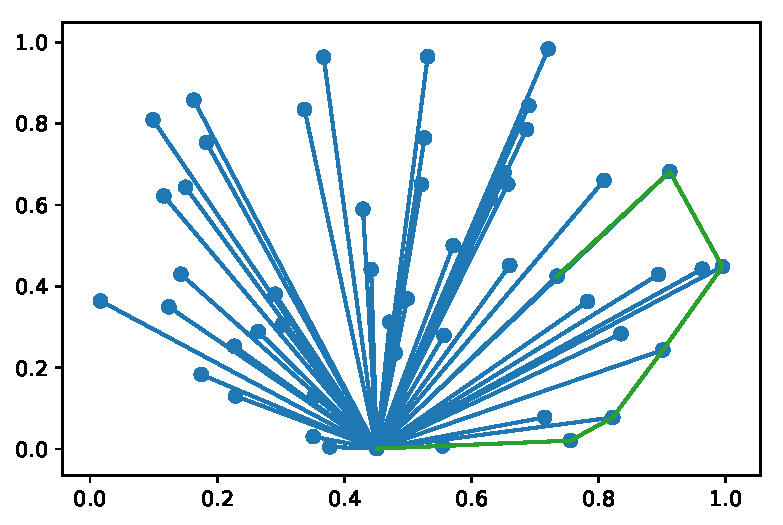
\includegraphics[width=.3\linewidth]{chull_10.python.pdf}}\hfill
 \subfloat[After 20 tested points.]{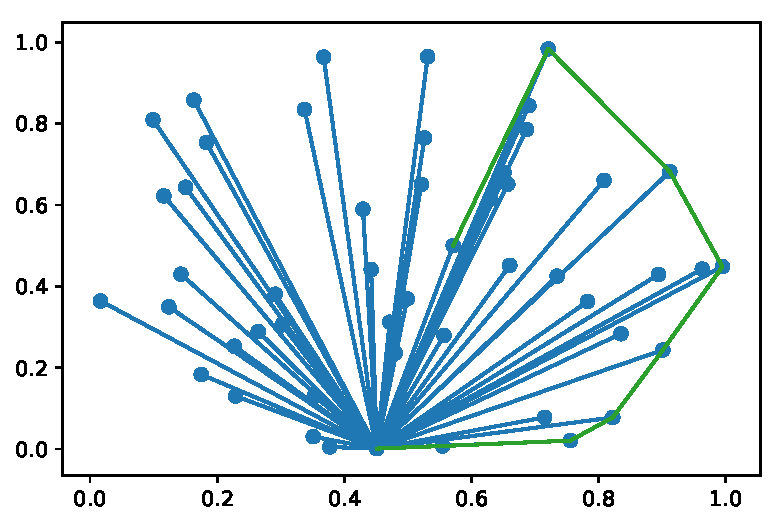
\includegraphics[width=.3\linewidth]{chull_20.python.pdf}}\hfill
 \subfloat[After 30 tested points.]{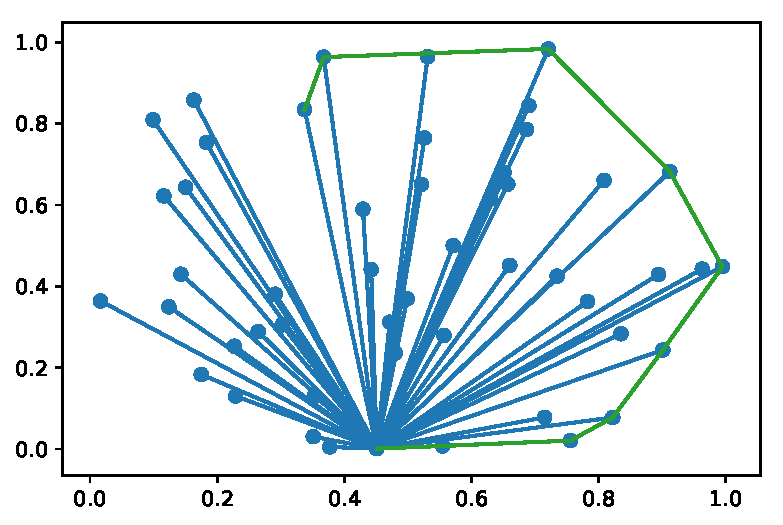
\includegraphics[width=.3\linewidth]{chull_30.python.pdf}}%
 \label{fig:python:convexhull:pause}%
 \vspace*{-10pt}%
\end{figure}

\subsection{Useful functions}

The cross-product function first extract the last two points of the hull, and check if there is a left-turn or a right-turn to go to the point $p_3$.
\begin{python}
def crossProduct(hull, p3):
    """
    Cross product
    hull : list that should contain at least 2 points
    p3   : point
    """
    p1 = hull[-2];
    p2 = hull[-1];
    
    c= (p2[0] - p1[0])*(p3[1] - p1[1]) - (p3[0] - p1[0])*(p2[1] - p1[1]);
    return c;
\end{python}

In order to display the results, one function is proposed.
\begin{python}
def displayPointsAndHull(points, P, hull, filename=None):
    """
    Fonction for display points and hull
    optionally save figure into pdf file
    """
    fig = plt.figure();
    if P is not(None):
        for i in np.arange(points.shape[0]):
            plt.plot([P[0],points[i,0]], [P[1],points[i,1]], 'C0');
    plt.scatter(points[:,0], points[:,1]);
    
    hull = np.array(hull);
    plt.plot(hull[:,0], hull[:,1], 'C2');
    plt.show()
    if filename:
        fig.savefig(filename, bbox_inches='tight');
\end{python}


\subsection{Simple tests}
For 5 points:
\begin{python}
Points=np.array([[ 1,  2],
       [ 1, -4],
       [ 2, -1],
       [ 3, -4],
       [ 4,  1],
       [ 3,  0]])

H = conv_hull(Points);
displayPointsAndHull(Points, H, 'sample_hull.python.pdf');
\end{python}

For a few random points:
\begin{python}
nb=50;
Points = np.random.rand(nb, 2);
H = conv_hull(Points);
displayPointsAndHull(Points, H, 'random_hull.python.pdf');
\end{python}

The results are illustrated in Fig.\ref{fig:python:convexhull:res}.

\begin{figure}[htbp]
\centering\caption{Illustration of the convex hull computation.}%
\subfloat[Convex points of 5 points.]{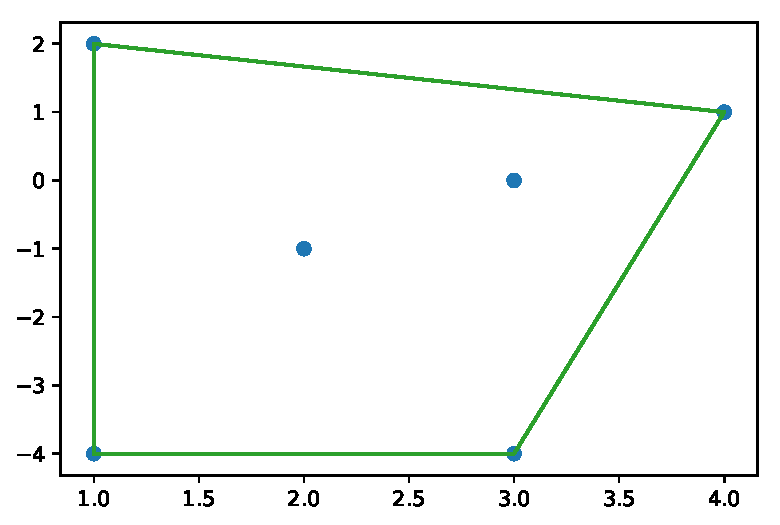
\includegraphics[width=.45\linewidth]{sample_hull.python.pdf}}\hfill
\subfloat[Convex hull of 50 random points.]{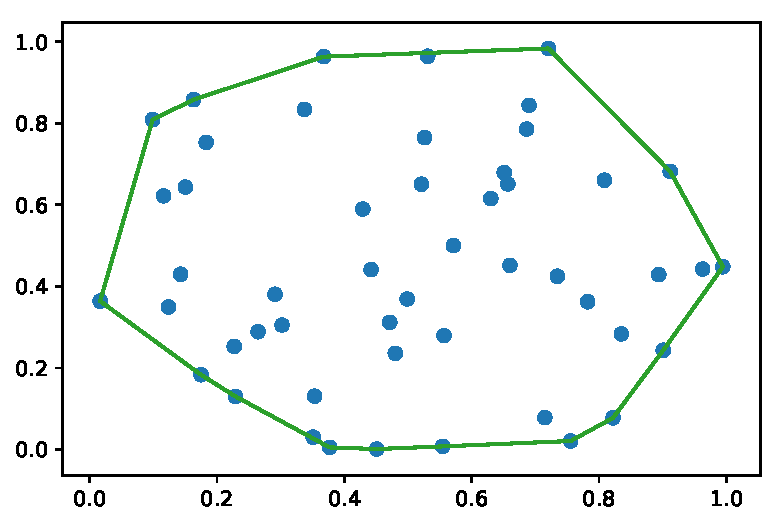
\includegraphics[width=.45\linewidth]{random_hull.python.pdf}}%
\label{fig:python:convexhull:res}%
\end{figure}


